\documentclass[10pt]{article}
\pdfoutput=1
%\usepackage{NotesTeX,lipsum}
\usepackage{NotesTeX,lipsum}

%\usepackage{showframe}

\title{\begin{center}{\Huge \textit{Notes}}\\{{\itshape Statistical Mechanics}}\end{center}}
\author{Yi Huang\footnote{\href{https://yiihuang.com/}{\textit{My Personal Website}}}}


\affiliation{
University of Minnesota
}

\emailAdd{yihphysics@gmail.com}

\begin{document}
	\maketitle
	\flushbottom
	\newpage
	\pagestyle{fancynotes}
	\part{Caprice}
	\section{Fall 2018}\label{sec: fall2018}
	%\section{Homework}\label{sec: homework}
	\begin{margintable}\vspace{.8in}\footnotesize
		\begin{tabularx}{\marginparwidth}{|X}
			Section~\ref{sec: fall2018}. Fall 2018\\
			Section~\ref{sec: homework}. Homework\\
		\end{tabularx}
	\end{margintable}

	This section is based on my course of statistical mechanics in Fall 2018 taught by Professor Kapusta. The textbook we use is Schwabl's \textit{Statistical Mechanics}. I also refer to Bellac's \textit{Equilibrium and Non-Equilibrium Statistical Thermodynamics}.

	\subsection{Proof of (1.4.12)}
	\begin{proof}
		We use the fact that trace of a matrix is invariant under change of basis.
		\begin{align*}
		\langle A \rangle_t &= \mathrm{Tr}(\rho(t) A) \\
		&= \mathrm{Tr}(U \rho(t_0) U^{\dagger} A) \\
		&= \mathrm{Tr}(U^{\dagger} (U \rho(t_0) U^{\dagger} A) U) \\
		&= \mathrm{Tr}(\rho(t_0) U^{\dagger} A U) \\
		&= \mathrm{Tr}(\rho(t_0) A_H(t))
		\end{align*}
	\end{proof}

	\subsection{Macroscopic systems are in general in mixed states}

	Consider a system consisting of two subsystems 1 and 2, and in a pure state
	\begin{gather}
		|\psi\rangle = \sum_{n,m}c_{nm} |1n\rangle |2m\rangle
	\end{gather}


	\subsection{Problem 1.14}

	Let $Y = \mathrm{ln}X$ be a  random variable obeys a Gaussian distribution, then $X = X(Y) = e^{Y}$ is a function of $Y$, with the probability density
	\begin{align*}
		\omega_{X}(x) &= \langle \delta(X(Y) - x) \rangle \\
		&= \int dy \, \omega_Y(y) \delta(e^y - x) \\
		&= \int dy \, \omega_Y(y) \frac{\delta(y - \mathrm{ln}x)}{|x|} \\
		& = \frac{1}{x \sqrt{2\pi \sigma^2}} e^{-\frac{(\mathrm{ln}(x/x_0))^2}{2 \sigma^2}}, \quad 0<x<\infty
	\end{align*}


	\subsection{Counter Intuition Fact about High-Dimensional Ball}

	Nearly the whole volume of a high-dimensional ball lies at its surface.

	The volume of a $N$ dimensional ball
	\begin{equation}
		V_N(r) = \frac{\pi^{N/2}}{\Gamma(\frac{N}{2}+1)}r^N,
	\end{equation}

	The surface area of a $N$ dimensional ball (area of $S_N$ surface)
	\begin{equation}
		S_N(r) = \frac{2 \pi^{N/2}}{\Gamma(\frac{N}{2})}r^{N-1},
	\end{equation}

	Suppose the thickness of this hypersphere is $\Delta r$, set the shell volume equal to the total ball volume to find the required $\Delta r$
	\begin{align*}
		S_N(r) \Delta r = V_N(r), \\
		\Delta r = \frac{V_N(r)}{S_N(r)} = \frac{r}{N}.
	\end{align*}

	For finite radius $r$, as the dimension gets higher and higher, say $N \to \infty$, then the ratio between the thickness and the radius goes to zero,
	\begin{equation}
		\frac{\Delta r}{r} = \frac{1}{N} \to 0,
	\end{equation}

	which means almost all the volume of this hypersphere lies on its surface.

	As for how to calculate the volume and the surface area of a $N$-dimensional ball, we can consider a Gaussian integral
	\begin{equation}
		G(N) = \int \dd x_1 \dd x_2 \dots \dd x_N \exp\left(-\sum_{i=1}^{N} x_i^2\right),
	\end{equation}

	Actually it is easy to get the result
	\begin{equation}
		G(N) = \left(\int_{-\infty}^{\infty} \dd x e^{-x^2}\right)^N = \pi^{N/2},
	\end{equation}

	However we can also compute this integral in polar coordinate
	\begin{align*}
	G(N) &= \int_0^{\infty} \dd r \int_{S_N(r)} \dd S_N(r) e^{-r^2} \\
	&= \int_0^{\infty} \dd r \, S_N(r) e^{-r^2},
	\end{align*}

	Although we don't know what is $S_N(r)$, what we do know is
	\begin{gather}
		V_N(r) = V_N(1)r^N, \\
		S_N(r) = \frac{\dd V_N(r)}{\dd r} = NV_N(1)r^{N-1}.
	\end{gather}

	Substitute into $G(N)$
	\begin{align*}
		G(N) &= NV_N(1) \int_0^{\infty} \dd r \, r^{N-1} e^{-r^2} \\
		&= \frac{1}{2}NV_N(1) \int_0^{\infty} \dd (r^2) \, (r^2)^{N/2-1} e^{-r^2} \\
		&= \frac{1}{2}NV_N(1) \int_0^{\infty} \dd z \, z^{N/2-1} e^{-z} \\
		&= \frac{1}{2}NV_N(1) \Gamma(N/2).
	\end{align*}

	Here we use the definiton of Gamma function
	\begin{equation}
		\Gamma(t) = \int_0^{\infty} \dd z \, z^{t-1}e^{-z}.
	\end{equation}
	Thus we have
	\begin{equation}
		\frac{1}{2}NV_N(1) \Gamma(N/2) = \pi^{N/2},
	\end{equation}
	which means
	\begin{equation}
		V_N(r) = \frac{\pi^{N/2}}{\Gamma(N/2 +1)}r^N,
	\end{equation}
	and
	\begin{equation}
		S_N(r) = \frac{2\pi^{N/2}}{\Gamma(N/2)}r^{N-1}
	\end{equation}

	\subsection{Derivation of (1.3.6)}

	Classically, the probability density in phase space is given by
	\begin{equation}
		\rho(q,p,t) = \int \dd q_0 \dd p_0 W(q_0, p_0) \delta(q - q(t;q_0,p_0)) \delta(p - p(t;q_0,p_0)).
	\end{equation}

	We want to calculate time derivative of $\rho$
	\begin{equation}
		\frac{\partial \rho}{\partial t} = \int \dd q_0 \dd p_0 W(q_0, p_0) \frac{\partial}{\partial t}[\delta(q - q(t;q_0,p_0)) \delta(p - p(t;q_0,p_0))].
	\end{equation}

	To compute this partial derivative, we use a property of derivative
	\begin{equation}
		\frac{\dd}{\dd x}v(x) = -\frac{\dd}{\dd x}v(-x),
	\end{equation}

	and
	\begin{equation}
		\frac{\dd}{\dd (x-L)}v(x-L) = \frac{\dd}{\dd x}v(x-L) = \frac{\dd}{\dd L}v(L-x) = - \frac{\dd}{\dd L}v(x-L).
	\end{equation}

	Thus
	\begin{align*}
		f(x,t) &= \int \dd x_0 \omega(x_0)\delta(x-q_x(t;x_0))\\
		\frac{\partial}{\partial t} f(x,t) &= \int \dd x_0 \omega(x_0) \frac{\partial (x-q_x(t;x_0))}{\partial t} \frac{\partial \delta(x-q_x(t;x_0))}{\partial (x-q_x(t;x_0))} \\
		&= - \int \dd x_0 \omega(x_0) \dot q_x(t;x_0) \frac{\partial \delta(x-q_x(t;x_0))}{\partial (x-q_x(t;x_0))}\\
		&= - \int \dd x_0 \omega(x_0) \dot q_x \frac{\partial}{\partial x}  \delta(x-q_x(t;x_0))\\
		&= - \dot x \frac{\partial}{\partial x} \int \dd x_0 \omega(x_0) \delta(x-q_x(t;x_0)) \\
		&= - \dot x \frac{\partial}{\partial x} f(x,t).
	\end{align*}

	Thus
	\begin{equation}
		\frac{\partial \rho}{\partial t} = -\sum_i\left(\dot{q_i} \frac{\partial}{\partial q_i} + \dot{p_i} \frac{\partial}{\partial p_i} \right) \rho
	\end{equation}

	\subsection{Proof of (2.3.5)}

	Entropy is defined by
	\begin{equation}
		S[\rho] = -k \, \mathrm{Tr}(\rho \, \mathrm{ln}\rho) = -k \langle\mathrm{ln} \rho \rangle.
	\end{equation}

	The entropy of microcanonical emsemble $S_{MC}$ is largest element of the entropy of any given density matrix. There is a theorem (2.3.3)
	\begin{equation}
		\mathrm{Tr}(\rho(\mathrm{ln} \rho_1 - \mathrm{ln} \rho)) < 0,
	\end{equation}

	if $\rho \neq \rho_1$.

	For microcanonical ensemble, $S[\rho_{MC}] = \mathrm{Tr}(\rho_{MC} \mathrm{ln} \rho_{MC}) = \mathrm{Tr}(\rho \mathrm{ln} \rho_{MC})$ is true for any density matrix $\rho$.

	So
	\begin{equation}
		S[\rho] = -k \, \mathrm{Tr}(\rho \, \mathrm{ln}\rho) \le -k \mathrm{Tr}(\rho \, \mathrm{ln}\rho_{MC}) = S_{MC},
	\end{equation}

	$S[\rho] = S_{MC}$ if and only if $\rho = \rho_{MC}$, which means $S_{MC}$ is the largest element of entropy.

	Notice that $-k \, \mathrm{Tr}(\rho \, \mathrm{ln}\rho_1)$ doesn't have physical meaning if $\rho \neq \rho_1$ but it is also an upper bound of $S[\rho]$, since
	\begin{equation}
		S[\rho] = -k \, \mathrm{Tr}(\rho \, \mathrm{ln}\rho) < -k \mathrm{Tr}(\rho \, \mathrm{ln}\rho_1)
	\end{equation}

	\subsection{How does statistical mechanics relate to probability theory?}

	The random variables in statistical mechanics are 3$N$ coordinates $q_i$ and 3$N$ canonical momentum $p_i$, $i = 1,2, \dots, 3N$. Also functions of these 6$N$ random variables are also random variables, for example, the Hamiltonian $H(q,p)$.

	Why are the 6$N$ degrees of freedom random variables?

	Because we cannot solve for a macroscopic system exactly in general when $N \to \infty$, nor even know the initial conditions. We should expect there is a distuibution function to assign probabilty to every point in the phase space. That's where the density matrix comes from.

	\subsection{Derivation of (2.6.3)}


	$\tilde{E}_1$ is the energy of subsystem 1 when the whole system is in the most probable state. Suppose when the overall system is at equilibrium state, $(\tilde{E}_1 - E_{1n})$ is much small compare to the energy of the heat bath $(E - \tilde{E}_1)$, so we can expand $\mathrm{ln}\Omega_2 $
	\begin{align*}
		\ln\Omega_2(E - E_{1n}) &= \ln\Omega_2(E - \tilde{E}_1 + \tilde{E}_1 - E_{1n}) \\
		&= \ln\Omega_2(E - \tilde{E}_1) + \left[\frac{\partial }{\partial(E - \tilde{E}_1)}\ln\Omega_2(E - \tilde{E}_1)\right]_{E - \tilde{E}_1}(\tilde{E}_1 - E_{1n}) \\
		&= \ln\Omega_2(E - \tilde{E}_1) + \frac{\tilde{E}_1 - E_{1n}}{kT}
	\end{align*}

	Therefore
	\begin{equation}
		\Omega_2(E - E_{1n}) = \Omega_2(E - \tilde{E}_1) \exp\left(\frac{\tilde{E}_1 - E_{1n}}{kT}\right).
	\end{equation}

	\subsection{Derivation of (2.6.12)}

	The partition function of canonical ensemble is
	\begin{align*}
		Z &= \mathrm{Tr_1}\exp(-H_1/kT) \\
		&= \int dE_1 \mathrm{Tr_1}\exp(-H_1/kT) \delta(H_1 - E_1) \\
		&= \int dE_1 \mathrm{Tr_1}\exp(-E_1/kT) \delta(H_1 - E_1) \\
		&= \int dE_1 \exp(-E_1/kT) \Omega_1(E_1).
	\end{align*}

	\subsection{An interesting derivative}

	Suppose $v(x_1 - x_2)$ is a fuction of relative position, then
	\begin{equation}
		\left(x_1 \frac{\partial}{\partial x_1} + x_2 \frac{\partial}{\partial x_2}\right) v(x_1 - x_2) = (x_1 - x_2) \frac{\partial v(x_1 - x_2)}{\partial (x_1 - x_2)}
	\end{equation}

	\subsection{Statistical Ensemble}

	\begin{remark}
		The collection of all the microstates which represent a macrostate, weighted by their frequency of occurrence, is referred to as a statistical ensemble. - page 3 in Schwabl's textbook.
	\end{remark}

	In this statement, he assumes that the frequency of occurrence of the time scale of measurement is equal to the probability of the microstates. Which means the number of microstate transitions during a measurement is really large. Suppose the microstate transition is driven by external perturbation, then this large number of transitions means the external perturbation happens at a pretty fast rate.

	\subsection{Density matrix in Schr\"{o}dinger picture and Heisenberg picture}

	The density matrix $\rho$ actually represents the property of states themselves, so in Sch\"{o}rdinger picture, $\rho$ is time-dependent, such that
	\begin{align*}
	\rho(t) &= \sum_i p_i |\psi_i(t) \rangle \langle \psi_i (t) | \\
	&= \sum_i p_i U(t,t_0)|\psi_i \rangle \langle \psi_i |U^{\dagger}(t,t_0)\\
	&= U(t,t_0) \rho(t_0) U^{\dagger}(t,t_0)
	\end{align*}

	However, in Heisenberg picture, $\rho$ should be time-independent.

	\subsection{Two equivalent statement of equilibrium statistical mechanics hypothesis}

	\begin{enumerate}
		\item An equilibrium state requires that
			\begin{equation}
				\dot{\rho} = \frac{\partial \rho}{\partial t} = -\frac{1}{i \hbar}[\rho, H] = 0,
			\end{equation}
		\item All microstates in the energy shell are equally probable.
	\end{enumerate}

	Next we prove they are equivalent, given the fact that ergodic hypothesis is true in classical case.
	\begin{itemize}
		\item 1 $\to$ 2: Classically, $\frac{\partial \rho}{\partial t} = 0$ has the physical meaning that for a fixed position in phase space, the probability density doesn't change as time goes by. Since the probability density are like incompressible flow and if you go with the trajectory in phase space, the probability density doesn't change according to Liouville theorem $\dot{\rho} =0$, the fact that you observe constant density at a fixed position implies before the probability density flows into this position, its magnitude is also the same constant. If ergodic hypothesis is true, the the phase trajectory pass by this position will "fill" the whole energy shell, such that the probability density for any position in this energy shell is equal. Quantum mechanically, If regions within the energy shell had different statistical weights, then the distribution function (density matrix) would depend on other quantities besides $H(q,p)$, and $\rho$ would not commute with $H$ (classically, the Poisson bracket would not vanish).

		\item 2 $\to$ 1: Classically, all states within the energy shell are equally probable means $\rho$ is inversely proportional to the volume of the energy shell, which is specified by the Hamiltonian $H$, and $\rho$ is a function of $H$. This implies the Poisson bracket $[\rho, H] = 0$. Quantum mechanically, the density matrix sums over the states within the energy shell, which is also specified by the Hamiltonian $H$. By the similar reason the commutator $[\rho, H] = 0$.
	\end{itemize}

	\subsection{A Thought}

	The classical mechanics are discovered in macroscopic world, where we cannot see all microscopic ``objects'', so it is kind of emergence phenomena or effective theory. However, when we want to write done the equation for microscopic objects, we borrow the classical ideas, for example the classical Hamiltonian, but why that is applicable? Is that amazing that the emergent classical effective theory can also describe the microscopic objects?

	\subsection{$TdS$ equation}

	The following equation of heat is valid only for quasi-static process
	\begin{equation}
		\delta Q = TdS.
	\end{equation}

	An infinitesimal reversable process doesn't change the entropy, thus $\delta Q = 0$. This is not true for a reversable process that forms a circle, and in this case, we require $\Delta S = 0$.

	\subsection{Legendre transformation}

	Since Legendre transformation only makes sense when the fucntion is convex or concave, does it means that in mechanics, Lagrangian and Hamiltonian must be convex or concave?

	\subsection{Property of $\delta$ function}
	\begin{theorem}
		\begin{equation}
			\int f(x) \delta(g(x)) \dd x = \sum_i \frac{f(x_i)}{|g(x_i)|},
		\end{equation}
		where $x_i$ are the roots of $g(x) = 0$.
	\end{theorem}
	\begin{proof}
		Change integration variable
		\begin{align*}
			\int_{g_{-\infty}}^{g_{\infty}} f(x) \delta(g(x)) \frac{\dd x}{\dd g(x)} \dd g(x)
			&= \int_{g_{-\infty}}^{g_{\infty}}   \frac{f(x)}{g'(x)} \delta(g(x)) \dd g(x) \\
			&= \sum_i \int_{g(x_i - \Delta)}^{g(x_i + \Delta)}   \frac{f(x)}{g'(x)} \delta(g(x)) \dd g(x), \numberthis \label{eq: delta function}
		\end{align*}
		where in \eqref{eq: delta function} $0 < \Delta \ll \min_{i\neq j}\{|x_i - x_j|\}$.
		If $g'(x_i)>0$, then $g(x_i + \Delta) > g(x_i - \Delta)$, so we obtain
		\begin{gather}
			\int_{g(x_i - \Delta)}^{g(x_i + \Delta)}   \frac{f(x)}{g'(x)} \delta(g(x)) \dd g(x) = \frac{f(x_i)}{g'(x_i)},
		\end{gather}
		If $g'(x_i)<0$, then $g(x_i + \Delta) < g(x_i - \Delta)$, so we obtain
		\begin{gather}
			\int_{g(x_i - \Delta)}^{g(x_i + \Delta)}   \frac{f(x)}{g'(x)} \delta(g(x)) \dd g(x) = -\frac{f(x_i)}{g'(x_i)}.
		\end{gather}

		From above, we conclude that
		\begin{equation}
			\int f(x) \delta(g(x)) \dd x = \sum_i \frac{f(x_i)}{|g(x_i)|}.
		\end{equation}
	\end{proof}

	\subsection{The partition function of ideal quantum gas}

	Consider a system of $N$ noninteracting identical particles, the Hamiltonian for the whole system is given by
	\begin{equation}
		H = \sum_{i=1}^{N} H_i,
	\end{equation}
	where $H_i$ is the single-particle Hamiltonian for the $i$th particle. Suppose the energy spectrum for the single-particle Hamiltonian is $\varepsilon_l$, where $l$ labels the value of the energy and all other quantum numbers necessary to specify the quantum state (see Bellac page 268). That is to say, energy levels that are degenerate but specified by different quantum numbers will be labelled by different values for $l$). Furthermore, for convenience, we choose the ground state level as the reference energy $\varepsilon_l = 0$.
	For identical particles, the energy level of the whole system $E$ is specified by the occupation number $n_l$ for each single-particle energy level $\varepsilon_l$, i.e., the number of particles in each energy level.
	\begin{equation}
		E_r = E\{ n_l \} = \sum_{l=0}^{\infty} n_l \varepsilon_l
	\end{equation}
	where we denote the configuration of particles as $r = \{ n_l \}$. The canonical partition function for $N$ identical independent particles subjected to the constraint $N = \sum_l n_l$ is then written as
	\begin{align*}
		Z_N &= \sum_{r} \exp(-\beta E_r) \\
		&= \sum_{\substack{\{n_l\} \\ \sum_l n_l = N}} \exp(-\beta E\{n_l\}) = \sum_{\substack{\{n_l\} \\
		\sum_l n_l = N}} \prod_{l=0}^{\infty} \exp(-\beta n_l \varepsilon_l) \numberthis \label{eq: Z_C}
	\end{align*}

	If for some state $\varepsilon_l$ there is no particle occupied at all, then $n_l = 0$ and in the product $\prod_{l=0}^{\infty}$ we are multipling by $1$. In practice, the constraint $N = \sum_l n_l$ is not easily taken into account. Therefore, instead of using the canonical partition function \eqref{eq: Z_C} it is more convenient to use the grand partition function where the number of particles is not fixed.
	\begin{align*}
		Z_{G}(T,V,\mu) &= \sum_{N=0}^{\infty} Z_N(V,T) \exp(-\beta \mu N) = \sum_{N=0}^{\infty} z^N Z_N(V,T) \\
		&= \sum_{N=0}^{\infty} \sum_{\substack{\{n_l\} \\
		\sum_l n_l = N}} \prod_{l=0}^{\infty} \left[ z^{n_l} \exp(-\beta n_l \varepsilon_l) \right] \numberthis \label{eq: Z_G}
	\end{align*}
 	This expression \eqref{eq: Z_G} can be simplified by exchanging the order of two summations.
	\begin{align*}
		\sum_{N=0}^{\infty} \sum_{\substack{\{n_l\} \\
		\sum_l n_l = N}} &\equiv \sum_{N=0}^{\infty} \sum_{\substack{\{n_l\} \\
		\text{no constraint}}} \delta_{N, \sum_l n_l} \\
		&\equiv \sum_{\substack{\{n_l\} \\
		\text{no constraint}}} \sum_{N=0}^{\infty} \delta_{N, \sum_l n_l} \equiv \sum_{\substack{\{n_l\} \\
		\text{no constraint}}} \equiv \sum_{\{n_l\}} \numberthis \label{eq: exchange sum}
	\end{align*}
	For a fixed configuration $\{ n_l \}$, the Kronecker delta contribues for only one value of $N = \sum n_l$, such that we can eliminate the summation over $N$. In \eqref{eq: exchange sum} we abbreviate the summation of all possible configuration $\{ n_l \}$ without constraint as $\sum_{\{n_l\}}$. Also we can write it as
	\begin{equation}
		\sum_{\{n_l\}} \equiv \prod_{l = 0}^{\infty} \quad \sum_{\text{All allowed} \, n_l}
	\end{equation}
	for bosons
	\begin{equation}
		\sum_{\{n_l\}} = \sum_{n_0 = 0}^{\infty} \sum_{n_1 = 0}^{\infty} \sum_{n_2 = 0}^{\infty} \dots
	\end{equation}
	for fermions
	\begin{equation}
		\sum_{\{n_l\}} = \sum_{n_0 = 0}^{1} \sum_{n_1 = 0}^{1} \sum_{n_2 = 0}^{1} \dots
	\end{equation}
	Therefore we can rewrite \eqref{eq: Z_G}
	\begin{equation}
		Z_G = \sum_{\{ n_l \}} \prod_l (z \e^{-\beta \varepsilon_l})^{n_l}
	\end{equation}
	The grand partition function is also given by the trace
	\begin{align*}
		Z_G &= \Tr[\e^{-\beta(\hat{H} - \mu \hat{N})}] = \sum_r \langle r | \e^{-\beta(\hat{H} - \mu \hat{N})} | r \rangle \\
		&= \sum_{\{ n_l \}} \exp\left[-\beta \sum_l ( \varepsilon_l - \mu)n_l \right] = \sum_{\{ n_l \}} \prod_l \exp\left[-\beta ( \varepsilon_l - \mu)n_l \right] \\
		&= \sum_{\{ n_l \}} \prod_l (z \e^{-\beta \varepsilon_l})^{n_l}
	\end{align*}
	where
	\begin{align}
		\hat{H} | r \rangle &= \left(\sum_l \varepsilon_l n_l\right) | r \rangle, \\
		\hat{N} | r \rangle &= \left(\sum_l \hat{n}_l\right) | r \rangle = \left(\sum_l n_l\right) | r \rangle.
	\end{align}
	We are now able to perform the sum in \eqref{eq: Z_G} over all the configuration independently.
	For bosons
	\begin{align*}
		Z_{G}(T,V, \mu) &= \sum_{\{ n_l \}} \prod_l (z \e^{-\beta \varepsilon_l})^{n_l} \\
		&= \sum_{n_0 = 0}^{\infty} \sum_{n_1 = 0}^{\infty} \sum_{n_2 = 0}^{\infty} \dots (z \e^{-\beta \varepsilon_0})^{n_0} (z \e^{-\beta \varepsilon_1})^{n_1} (z \e^{-\beta \varepsilon_2})^{n_2} \dots \\
		&= \left[ \sum_{n_0 = 0}^{\infty} (z \e^{-\beta \varepsilon_0})^{n_0} \right] \left[ \sum_{n_1 = 0}^{\infty} (z \e^{-\beta \varepsilon_1})^{n_1} \right] \dots \\
		&= \prod_{l=0}^{\infty} \sum_{n_l = 0}^{\infty} (z \e^{-\beta \varepsilon_l})^{n_l} =
		\prod_l \frac{1}{1 - \e^{-\beta(\varepsilon_l - \mu)}},
	\end{align*}
	The geometric series converges when $\mu < \varepsilon_0$. For fermions
	\begin{equation}
		Z_{G}(T,V, \mu) = \prod_{l=0}^{\infty} \sum_{n_l = 0}^{1} (z \e^{-\beta \varepsilon_l})^{n_l} =
		\prod_l \left(1 + \e^{-\beta(\varepsilon_l - \mu)}\right)
	\end{equation}
	Equivalently we can write the grand partition function of bosons and fermions in a close form
	\begin{equation}
		Z_G = \prod_l Z_l = \prod_l [1 \mp \e^{-\beta(\varepsilon_l - \mu)}]^{\mp 1}
	\end{equation}
	where $Z_l = [1 \mp \e^{-\beta(\varepsilon_l - \mu)}]^{\mp 1}$; $-$ is for bosons, $+$ is for fermions.

	\subsection{The average occupation number of ideal quantum gas}

	Consider a single-particle state $| l \rangle$, the average occupation number is given by
	\begin{align*}
		\langle \hat{n}_l \rangle &= \Tr(\hat{\rho}\, \hat{n_l}) = Z_G^{-1} \Tr[\e^{-\beta(\hat{H} - \mu \hat{N})} \hat{n_l}] \\
		&= Z_G^{-1} \sum_r \langle r| \e^{-\beta(\hat{H} - \mu \hat{N})} \hat{n_l} | r \rangle \\
		&= Z_G^{-1} \sum_{\{ n_q \}} \exp\left[-\beta \sum_q ( \varepsilon_q - \mu)n_q \right] n_l \\
		&= \frac{\sum_{\{ n_q \}} \e^{-\beta \sum_q ( \varepsilon_q - \mu)n_q} n_l}{\sum_{\{ n_q \}} \e^{-\beta \sum_q ( \varepsilon_q - \mu)n_q}}
		= \frac{\prod_q \sum_{n_q} \e^{-\beta (\varepsilon_q - \mu)n_q} n_l}{\prod_q \sum_{n_q} \e^{-\beta (\varepsilon_q - \mu)n_q}} \\
		&= \frac{\left(\prod_{q \neq l} Z_q\right) \sum_{n_l} \e^{-\beta (\varepsilon_l - \mu)n_l} n_l}{\left(\prod_{q\neq l} Z_q\right) \sum_{n_l} \e^{-\beta (\varepsilon_l - \mu)n_l}}
		= \frac{\sum_{n_l} \e^{-\beta (\varepsilon_l - \mu)n_l} n_l}{\sum_{n_l} \e^{-\beta (\varepsilon_l - \mu)n_l}}
	\end{align*}
	Therefore we can rewrite the average occupation number as the partial derivative of the sub-partition function or the grand partition function
	\begin{gather}
		\langle \hat{n}_l \rangle = \beta^{-1} \del{\ln Z_l}{\mu} = - \beta^{-1} \del{\ln Z_G}{\varepsilon_l} \\
		\langle \hat{n}_l \rangle = \frac{1}{\e^{\beta(\varepsilon_l - \mu)} \mp 1}
	\end{gather}

	\subsection{Maxwell-Boltzmann statistics}

	The canonical partition function of $N$ Maxwell-Blotzmann particles is
	\begin{equation}
		Z_N^{\mathrm{MB}} = \sum_{\sum n_l = N} \frac{\e^{-\beta \varepsilon_0 n_0}}{n_0 !} \dots \frac{\e^{-\beta \varepsilon_l n_l}}{n_l !} \dots \label{eq: MB Z_C}
	\end{equation}
	The $n_l !$ in the denominators can be understood as the fact that the MB particles are identical, so the state of the whole system would not be changed if permuting the $n_l$ particles in the single-particle state with energy $\varepsilon_l$.
	\begin{theorem}
		Multinomial theorem: For any positive integer $m$ and any nonnegative integer $N$, the multinomial formula tells us how a sum with $m$ terms expands when raised to an arbitrary power $N$:
		\begin{equation}
			(x_1 + x_2 + \dots + x_m)^N = \sum_{\sum n_l = N}
			\begin{pmatrix}
				N \\
				n_1, n_2, \dots, n_m
			\end{pmatrix}
			\prod_{l = 1}^{m} x_l^{n_l}
		\end{equation}
		where
		\begin{equation}
			\begin{pmatrix}
				N \\
				n_1, n_2, \dots, n_m
			\end{pmatrix}
			= \frac{N!}{n_1! \cdots n_m!}
		\end{equation}
	\end{theorem}
	According to multinomial theorem, we can simpify the MB canonical partition function \eqref{eq: MB Z_C} as follows
	\begin{align*}
		Z_N^{\mathrm{MB}} &= \sum_{\sum n_l = N} \frac{\left(\e^{-\beta \varepsilon_0}\right)^{n_0}}{n_0 !} \dots \frac{\left(\e^{-\beta \varepsilon_l}\right)^{n_l}}{n_l !} \dots \\
		&= \frac{1}{N!} \sum_{\sum n_l = N}
		\begin{pmatrix}
			N \\
			n_0, \dots, n_l, \dots
		\end{pmatrix}
		\prod_l \left(\e^{-\beta \varepsilon_l}\right)^{n_l} \\
		&= \frac{1}{N!} \left(\sum_l \e^{-\beta \varepsilon_l}\right)^{N} \\
		&= \frac{(Z_1^{\mathrm{MB}})^N}{N!}
	\end{align*}
	where $Z_1^{\mathrm{MB}}$ is the partition function for a single-particle system
	\begin{equation}
		Z_1^{\mathrm{MB}} = \sum_{l=0}^{\infty} \e^{-\beta \varepsilon_l}
	\end{equation}
	Next we calculate the grand partition function
	\begin{equation}
		Z_G^{\mathrm{MB}} = \sum_{N=0}^{\infty} z^N Z_N^{\mathrm{MB}} = \sum_{N=0}^{\infty} z^N \frac{(Z_1^{\mathrm{MB}})^N}{N!} = \exp\left(z Z_1^{\mathrm{MB}}\right)
	\end{equation}

	\subsection{Riemann Zeta function}

	Riemann Zeta function is defined as the sum of the following infinite series
	\begin{equation}
		\zeta(\nu) = \sum_{k=1}^{\infty} \frac{1}{k^{\nu}},
	\end{equation}
	Notice that $\zeta(1)$ is known as the harmonic series. The fact that the harmonic series diverges was first proven in the 14th century by Nicole Oresme. His way to prove divergence is to compare the harmonic series with another divergent series, where each denominator is replaced with the next-largest power of two
	\begin{align*}
		\lefteqn{1 + \frac{1}{2} + \frac{1}{3} + \frac{1}{4} + \frac{1}{5} + \frac{1}{6} + \frac{1}{7} + \frac{1}{8} + \dots} \\
		&> 1 + \frac{1}{2} + \left(\frac{1}{4} + \frac{1}{4}\right) + \left(\frac{1}{8} + \frac{1}{8} + \frac{1}{8} + \frac{1}{8}\right) + \dots \\
		&= 1 + \frac{1}{2} + \frac{1}{2} + \frac{1}{2} + \dots
	\end{align*}
	Inspired by this comparison test, we can also consider the power of any other integer $k$, such that we seperate the whole series into segaments with $k^{n} - k^{n-1} = (k-1)k^{n-1}$ terms, and replace their denominator with $k^{n}$, the largest power of $k$ in this segament, such that
	\begin{align*}
		\lefteqn{\frac{1}{k^{n-1} +1} + \frac{1}{k^{n-1} + 2} + \dots + \frac{1}{k^n}}\\
		&> \frac{1}{k^n} + \frac{1}{k^n} + \dots + \frac{1}{k^n} = \frac{k-1}{k}
	\end{align*}
	There are infinite these segments in the harmonic series, so harmonic series is divergent
	\begin{align*}
		\sum_{l=1}^{\infty} &= \sum_{n=1}^{\infty} \sum_{i=1}^{(k-1)k^{n-1}} \frac{1}{k^{n-1} + i}\\
		&> \sum_{n=1}^{\infty} \sum_{i=1}^{(k-1)k^{n-1}} \frac{1}{k^n} \\
		&= \sum_{n=1}^{\infty} \frac{k-1}{k} = \frac{k-1}{k} \sum_{n=1}^{\infty} 1
	\end{align*}
	Next we consider $\zeta(2)$ which is also known as the Basel problem, first posed by Pietro Mengoli in 1650 and solved by Leonhard Euler in 1734.
	\begin{equation}
		\zeta(2) = 1 + \frac{1}{2^2} + \frac{1}{3^2} + \dots
	\end{equation}
	The Basel problem had withstood the attacks of the leading mathematicians of the day, including the Bernoulli family, but none of them succeeded. This ice was broken by Euler, who was a student of Bernoulli. Euler's solution brought him immediate fame when he was twenty-eight.

	Similar to our previous strategy, we can prove that this series is convergent
	\begin{align*}
		\lefteqn{1 + \left( \frac{1}{2^2} + \frac{1}{3^2} \right) + \left( \frac{1}{4^2} + \dots + \frac{1}{7^2} \right) + \left( \frac{1}{8^2} + \dots + \frac{1}{15^2} \right) + \dots} \\
		&< 1 + \left( \frac{1}{2^2} + \frac{1}{2^2} \right) + \left( \frac{1}{4^2} + \dots + \frac{1}{4^2} \right) + \left( \frac{1}{8^2} + \dots + \frac{1}{8^2} \right) + \dots\\
		&= 1 + \frac{1}{2} + \frac{1}{2^2} + \frac{1}{2^3} + \dots = \frac{1}{1 - 1/2} = 2
	\end{align*}
	But what is the exact value of $\zeta(2)$? Euler looked at this problem for quite a long time, and he finally figured out an amazing and creative way to solve it. His starting point is that the infinite summation can be related to the factorization of polynomial. For example, let's look at a quadratic polynomial
	\begin{align*}
		\lefteqn{\left(1- \frac{x}{\alpha_1}\right) \left(1- \frac{x}{\alpha_2}\right)} \\
		&= 1 - a x + b x^2 \\
		&= 1 - \left(\frac{1}{\alpha_1} + \frac{1}{\alpha_2}\right)x + \frac{1}{\alpha_1 \alpha_2}
	\end{align*}
	where $\alpha_{1,2}$ are two roots of the polynomial $1 - a x + b x^2$, and $a = \tfrac{1}{\alpha_1} + \tfrac{1}{\alpha_2}$. By the same token, we should consider a polynomial of order $2n$ with roots $\pm1, \pm2, \dots, \pm n$
	\begin{align*}
		\lefteqn{\left( 1 - \frac{x}{1} \right)\left( 1 + \frac{x}{1} \right) \left( 1 - \frac{x}{2} \right)\left( 1 + \frac{x}{2} \right) \cdots \left( 1 - \frac{x}{n} \right)\left( 1 + \frac{x}{n} \right)} \\
		&= 1 - \left( \frac{1}{1^2} + \frac{1}{2^2} + \dots + \frac{1}{n^2} \right) x + \dots
	\end{align*}
	In order to calculate $\zeta(2)$, we need to find a polynomial whose roots lie in $\pm 1, \pm 2, \dots$. Since this polynomial is of infinite order, we should consider the taylor expandsion of some function which can represent this polynomial. According to our knowledge of the shape of functions, $\sin x$ has roots $0, \pm \pi, \pm 2\pi, \dots$, so it is natural to propose the following conjecture
	\begin{align*}
		\sin x &= C x \left( 1 - \frac{x}{\pi} \right)\left( 1 + \frac{x}{\pi} \right) \left( 1 - \frac{x}{2\pi} \right)\left( 1 + \frac{x}{2\pi} \right) \cdots \\
		&= C x \prod_{n=1}^{\infty} \left[ 1 - \frac{x^2}{(n\pi)^2} \right] \numberthis \label{conj: sinx/x}
	\end{align*}
	where $C$ is a constant which can be determined by the limit $x \to 0$
	\begin{equation}
		C = \lim_{x \to 0} \frac{\sin x}{x} = 1
	\end{equation}
	If conjecture~\eqref{conj: sinx/x} is true, we can obtain the exact value of $\zeta(2)$ by comparing the coefficient of $\sin x/x$
	\begin{equation}
		\frac{\sin x}{x} = \sum_{k=0}^{\infty} (-)^k \frac{x^{2k+1}}{(2k+1)!} = 1 - \frac{1}{3!} x^2 + \frac{1}{5!} x^5 + \dots \label{eq: taylor sinx/x}
	\end{equation}
	Therefore
	\begin{equation}
		\frac{1}{1^2\pi^2} + \frac{1}{2^2\pi^2} + \dots = \frac{1}{\pi^2}\left(\frac{1}{1^2} + \frac{1}{2^2} + \dots \right) = \frac{1}{6}
	\end{equation}
	or equivalently
	\begin{equation}
		\zeta(2) = \frac{\pi^2}{6}
	\end{equation}
	Actually Euler's method is not restricted in calculating $\zeta(2)$, it can be generalized to calculate $\zeta(2n)$ for all even powers. To do this, we should consider a infinite order polynomial which can be factorized as an infinite series
	\begin{equation}
		1 + A_1 z + A_2 z^2 + A_3 z^3 + \dots = (1 + \alpha_1 z) (1 + \alpha_2 z) (1 + \alpha_1 z)(1 + \alpha_3 z) \cdots
	\end{equation}
	Now we want to get the summation of every power of $\alpha_i$ as follows
	\begin{align*}
		S_1 &= \alpha_1 + \alpha_2 + \alpha_3 + \dots, \\
		S_2 &= \alpha_1^2 + \alpha_2^2 + \alpha_3^2 + \dots, \\
		S_3 &= \alpha_1^3 + \alpha_2^3 + \alpha_3^3 + \dots, \\
		&\vdots
	\end{align*}
	By comparing the coefficients we obtained
	\begin{align*}
		S_1 &= A_1, \\
		S_2 &= A_1 S_1 - 2 A_2,\\
		S_3 &= A_1 S_2 - A_2 S_1 + 3 A_3, \\ \numberthis \label{eq: S_3}
		&\vdots
	\end{align*}
	\begin{proof}
		Expand the infinite series as polynomial
		\begin{equation}
			\prod_{i=1}^{\infty} (1 + \alpha_i z) = 1 + \left(\sum_i \alpha_i \right) z + \left(\sum_{i < j} \alpha_i \alpha_j \right) z^2 + \left(\sum_{i < j < k} \alpha_i \alpha_j \alpha_k \right) z^3 + \dots
		\end{equation}
		Therefore the expression of $A_i$ are given by
		\begin{align*}
			A_1 &= \sum_i \alpha_i,\\
			A_2 &= \sum_{i < j} \alpha_i \alpha_j, \\
			A_3 &= \sum_{i < j < k} \alpha_i \alpha_j \alpha_k, \\
			&\vdots
		\end{align*}
		Obviously $S_1 = A_1$. Next we need to prove $S_2 = A_1 S_1 - 2 A_2$
		\begin{align*}
			A_1 S_1 &= \left( \sum_i \alpha_i \right) \left( \sum_j \alpha_j \right) \\
			&= \left( \sum_{i=j} + \sum_{i \neq j} \right) \\
			&= \sum_i \alpha_i^2 + 2\sum_{i < j} \alpha_i \alpha_j
		\end{align*}
		Therefore
		\begin{equation}
			A_1 S_1 - 2 A_2 = \sum_i \alpha_i^2 + 2\sum_{i < j} \alpha_i \alpha_j - 2\sum_{i < j} \alpha_i \alpha_j = \sum_i \alpha_i^2 = S_2
		\end{equation}
		For $S_3 = A_1 S_2 - A_2 S_1 + 3 A_3$, we calculate the right hand side of the equation by each term
		\begin{align*}
			A_1 S_2 &= \left( \sum_i \alpha_i \right) \left( \sum_j \alpha_j^2 \right) \\
			&= \left(\sum_{i=j} + \sum_{i \neq j} \right) \alpha_i \alpha_j^2 \\
			&= \sum_i \alpha_i^3 + \sum_{i \neq j} \alpha_i \alpha_j^2,
		\end{align*}
		and
		\begin{align*}
			A_2 S_1 &= \left( \sum_{i < j} \alpha_i \alpha_j \right) \left( \sum_k \alpha_k \right) \\
			&= \left(\sum_{i < j=k} + \sum_{k= i < j} + \sum_{i<j<k} + \sum_{i<k<j} + \sum_{k<i<j}\right) \alpha_i \alpha_j \alpha_k \\
			&= \sum_{i \neq j}\alpha_i \alpha_j^2 + 3 \sum_{i<j<k} \alpha_i \alpha_j \alpha_k,
		\end{align*}
		Thus the right hand side of \eqref{eq: S_3} is given by
		\begin{align*}
			\lefteqn{A_1 S_2 - A_2 S_1 + 3 A_3} \\
			&= \sum_i \alpha_i^3 + \sum_{i \neq j} \alpha_i \alpha_j^2 - \sum_{i \neq j}\alpha_i \alpha_j^2 - 3 \sum_{i<j<k} \alpha_i \alpha_j \alpha_k + 3 \sum_{i<j<k} \alpha_i \alpha_j \alpha_k \\
			&= \sum_i \alpha_i^3 = S_3
		\end{align*}
		The key point to calculate the above terms is changing double summations into a single summation with different constraints.
	\end{proof}
	In our case, we choose the polynomial as $\sin x /x$ and consider the coefficients of all even powers of $x$, then
	\begin{align*}
		\zeta(2) &= 1 + \frac{1}{2^2} + \frac{1}{3^2} + \dots = - \pi^2 S_1, \\
		\zeta(4) &= 1 + \frac{1}{2^4} + \frac{1}{3^4} + \dots = \pi^4 S_2, \\
		\zeta(6) &= 1 + \frac{1}{2^6} + \frac{1}{3^6} + \dots = - \pi^6 S_3, \\
		&\vdots \\
		\zeta(2n) &= (-\pi^2)^n S_n
	\end{align*}
	From \eqref{eq: taylor sinx/x}, we know that $A_n = (-)^n 1/(2n+1)!$, so we can compute $S_n$ as follows
	\begin{align*}
		S_1 &= A_1 = -\frac{1}{3!} = -\frac{1}{6} = \frac{(2\pi)^{2}}{2(2!)} \frac{1}{6}, \\
		S_2 &= A_1 S_1 - 2 A_2 =  \left(-\frac{1}{3!}\right)\left(-\frac{1}{3!}\right) - 2 \frac{1}{5!} = \frac{1}{90} = \frac{(2\pi)^{4}}{2(4!)} \frac{1}{30}, \\
		S_3 &= A_1 S_2 - A_2 S_1 + 3 A_3 \\
		&= \left(-\frac{1}{3!}\right) \frac{1}{90} - \frac{1}{5!} \left(- \frac{1}{6} \right) + 3 \left(-\frac{1}{7!}\right) \\
		&= -\frac{1}{945} = \frac{(2\pi)^{6}}{2(6!)} \frac{1}{42}
	\end{align*}
	Therefore
	\begin{align*}
		\zeta(2) &= - \pi^2 S_1 = \frac{\pi^2}{6}, \\
		\zeta(4) &= \pi^4 S_2 = \frac{\pi^4}{90}, \\
		\zeta(6) &= - \pi^6 S_3 = \frac{\pi^6}{945}, \\
		&\vdots \\
		\zeta(2n) &= (-\pi^2)^n S_n = \ ?
	\end{align*}
	Later we will prove that $\zeta(2n)$ is related to Bernoulli number $B_{2n}$.
	\begin{theorem}
		\begin{equation}
			\zeta(2n) = (-)^{n+1} \frac{(2\pi)^{2n} B_{2n}}{2(2n)!}
		\end{equation}
	\end{theorem}
	The above results are valid if our conjecture \eqref{conj: sinx/x} is true. We haven't prove that it is true! Don't worry, as one of the greatest mathematician, Euler proved this conjecture 200 years ago, or we should rewrite it as a theorem since it's been proven.
	\begin{theorem} \label{th: sin prod}
		\begin{equation}
			\sin x = x \prod_{n=1}^{\infty} \left[ 1 - \frac{x^2}{(n\pi)^2} \right]
		\end{equation}
	\end{theorem}
	\begin{proof}
		It seems like we have already prove theorem \ref{th: sin prod} from the perspective of factorization of polynomial, but it is not rigorous because we do not know whether the infinite product converges or not.
	\end{proof}

	\newpage

	\section{Homework}\label{sec: homework}

	\subsection{Homework 7}
	\begin{enumerate}
		\item Calculate the second virial coefficient for the soft-core potential
		\begin{equation}
			v_2(r) =
			\begin{cases}
				u_0 & \qif 0 < r < r_0, \\
				-u_1 & \qif r_0 < r < r_1, \\
				0 & \qif r > r_1,
			\end{cases}
		\end{equation}
		where $u_{0,1}$ are both positive.

		By definition the second virial coefficient is given by
		\begin{align}
			B_2 &= -\half \int \dd^3 r \qty(\e^{-\beta v_2(r)} - 1) \\
			&= -\half \qty[\frac{4\pi r_0^3}{3}(\e^{-\beta u_0} - 1) + \frac{4\pi (r_1^3 - r_0^3)}{3}(\e^{\beta u_1} - 1)].
		\end{align}
		\item Do a least squares fit of the virial coefficient you calculated in problem 1 to the data on nitrogen which can be found in the \href{http://www.ddbst.com/en/EED/PCP/BII_C1056.php}{Dortmund Data Bank}. See Fig. \ref{fig: virial fit}.
		\begin{figure}[htbp]
			\centering
			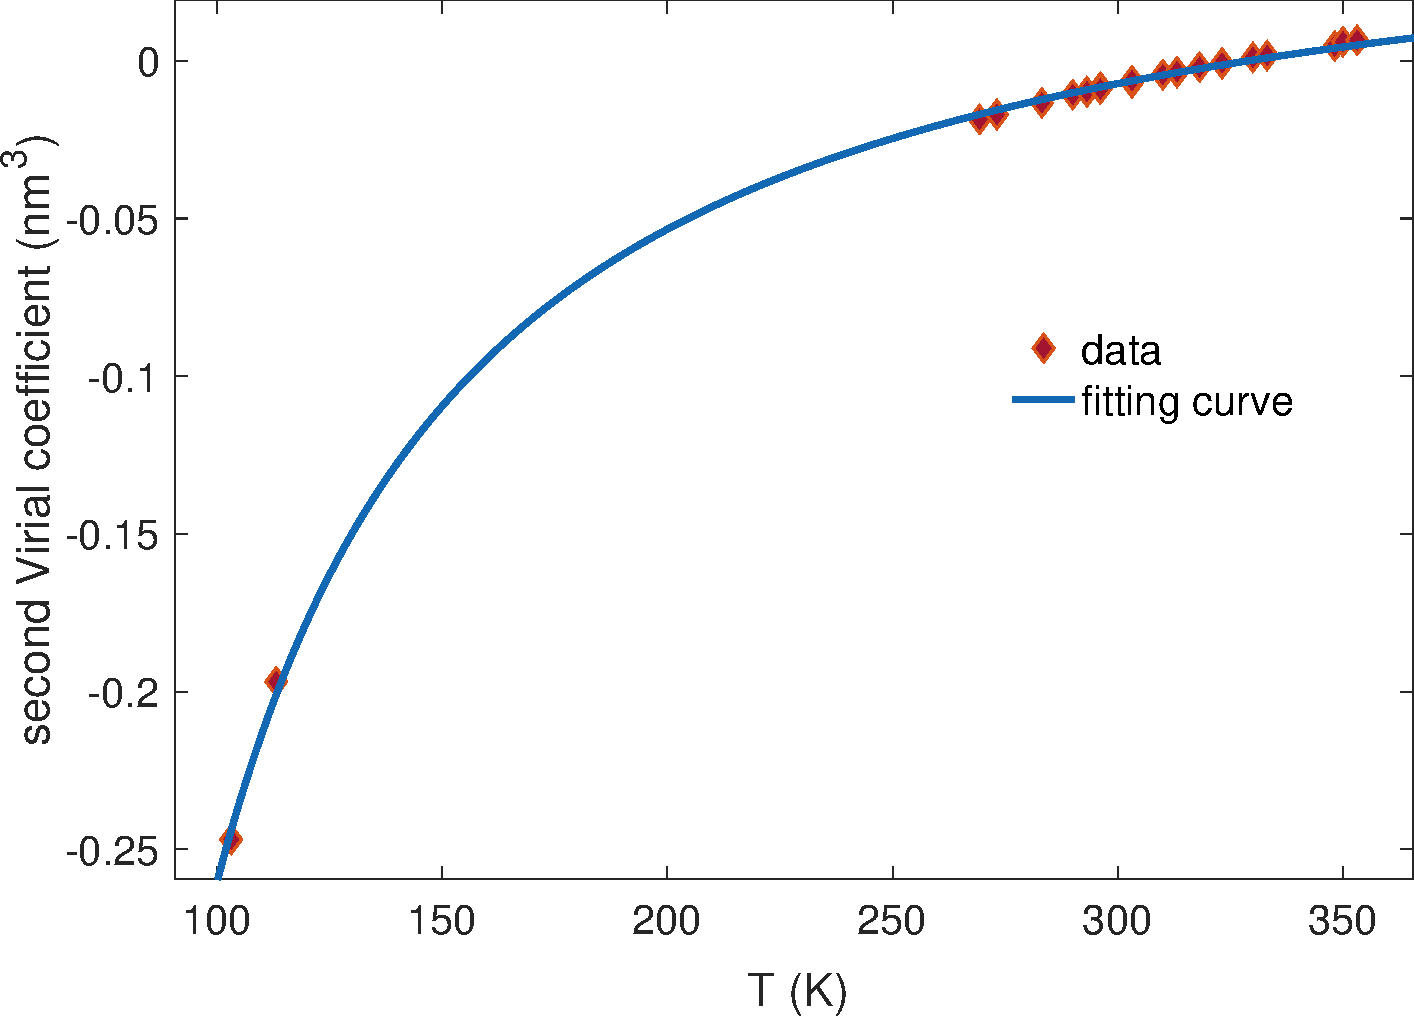
\includegraphics[width=0.7 \textwidth]{figure/virial_fit.pdf}
			\caption{This is a nonlinear least squares fit of the virial coefficient to the data of nitrogen. The fit values of each parameters are $u_0 = 0.8464 \eV$, $u_1 = 0.01007 \eV$, $r_0 = 0.3094 \nm$, and $r_1 = 0.4626 \nm$. The root-mean-square error of this fitting curve is 0.001428, with $R^2 = 0.9995$.}
			\label{fig: virial fit}
		\end{figure}
	\end{enumerate}



	\newpage

\end{document}
